\documentclass[letterpaper]{article}
\usepackage{settings}

\begin{document}
\begin{notes}{Part 4: Geometric Transformations and Warping}

\NoteChapter{Geometric Transformation}

\textbf{Geometric transformations} map points from one image (or coordinate frame) to another. They form a strict hierarchy: each class is a special case of the one below it, preserving strictly more geometric structure.

\NoteSection{Homogeneous Coordinates}

A 2D point $(x,y)$ is embedded in homogeneous coordinates as the equivalence class $(\tilde x, \tilde y, \tilde w) \sim \lambda(\tilde x,\tilde y,\tilde w)$ for any $\lambda\neq0$, representing the Euclidean point $(x,y)=(\tilde x/\tilde w,\,\tilde y/\tilde w)$. The canonical representative uses $\tilde w=1$: $(x,y,1)^T$. Points at infinity have $\tilde w=0$ and represent directions.\\

\textbf{Why homogeneous coordinates?} Every transformation in the hierarchy below - including \emph{translation} - becomes a linear (matrix) map on homogeneous coordinates. This allows composing any sequence of transformations by simply multiplying their $3\times3$ matrices.


\NoteSection{2D Transformations}

\NoteSubsection{2D Transformations and Their Hierarchy}

\begin{figure}[H]
    \centering
    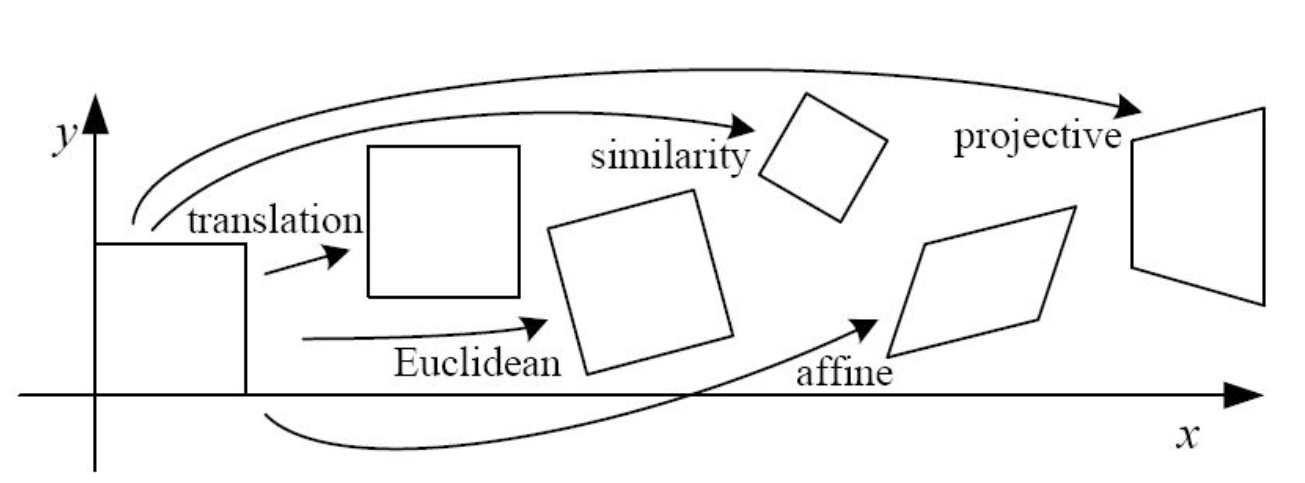
\includegraphics[width=0.9\linewidth]{images/part4/geometric-transformations.png}
\end{figure}

\textbf{Translation (2 DOF.)} Shifts the origin; no rotation or distortion.
$$\mathbf{x}' = \mathbf{x} + \mathbf{t}, \qquad \begin{bmatrix}x'\\y'\\1\end{bmatrix} = \begin{bmatrix}1&0&t_x\\0&1&t_y\\0&0&1\end{bmatrix}\begin{bmatrix}x\\y\\1\end{bmatrix}.$$
\emph{Invariants:} all distances, angles, areas, parallelism, and lengths.\\

\textbf{Euclidean/Rigid (3 DOF.)} Rotation $\theta$ plus translation; preserves the shape of objects.
$$\mathbf{x}' = R\mathbf{x}+\mathbf{t}, \qquad \begin{bmatrix}x'\\y'\\1\end{bmatrix} = \begin{bmatrix}\cos\theta&-\sin\theta&t_x\\\sin\theta&\cos\theta&t_y\\0&0&1\end{bmatrix}\begin{bmatrix}x\\y\\1\end{bmatrix},$$
where $R$ is defined to be the rotation matrix,
$$R=
\begin{bmatrix}
    \cos\theta&-\sin\theta& 0\\
    \sin\theta&\cos\theta& 0\\
    0&0&1
\end{bmatrix},
$$
$R\in SO(2)$ satisfies $RR^T=I$, $\det R=1$. \emph{Invariants:} all distances and angles (congruence).\\

\textbf{Similarity (4 DOF.)} Adds uniform scaling $s>0$ to the Euclidean transform.
$$\begin{bmatrix}x'\\y'\\1\end{bmatrix} = \begin{bmatrix}s\cos\theta&-s\sin\theta&t_x\\s\sin\theta&s\cos\theta&t_y\\0&0&1\end{bmatrix}\begin{bmatrix}x\\y\\1\end{bmatrix}.$$
\emph{Invariants:} angles, ratios of lengths, shape (but not absolute size). SIFT descriptors are designed to be similarity-invariant.\\

\textbf{Affine (6 DOF.)} Any invertible linear map plus translation; the last row is fixed to $[0,0,1]$.
$$\begin{bmatrix}x'\\y'\\1\end{bmatrix} = \begin{bmatrix}a_{11}&a_{12}&t_x\\a_{21}&a_{22}&t_y\\0&0&1\end{bmatrix}\begin{bmatrix}x\\y\\1\end{bmatrix} = \begin{bmatrix}A&\mathbf{t}\\\mathbf{0}^T&1\end{bmatrix}\begin{bmatrix}x\\y\\1\end{bmatrix},$$
where $A\in GL(2)$. An affine map can be decomposed as 
$$A = R(\theta)\,R(-\phi)\,\begin{bmatrix}\lambda_1&0\\0&\lambda_2\end{bmatrix}R(\phi)$$ 
(rotation $\to$ scale $\to$ un-rotate). \emph{Invariants:} parallelism, ratios of areas, ratios of lengths along parallel lines. Requires 3 point correspondences to estimate.\\

\textbf{Projective / Homography (8 DOF.)} The most general linear map on homogeneous coordinates; the last row is free (but $H$ is defined only up to a global scale factor, so $8$ free parameters).
$$\tilde{\mathbf{x}}' = H\tilde{\mathbf{x}}, \quad H = \begin{bmatrix}h_{11}&h_{12}&h_{13}\\h_{21}&h_{22}&h_{23}\\h_{31}&h_{32}&h_{33}\end{bmatrix},$$

$$\mathbf{x}' = \frac{1}{h_{31}x+h_{32}y+h_{33}}\begin{bmatrix}h_{11}x+h_{12}y+h_{13}\\h_{21}x+h_{22}y+h_{23}\end{bmatrix}.$$

\emph{Invariants:} straight lines and cross-ratio of four collinear points. A homography relates any two views of a planar surface (or two views taken from the same camera center). Requires 4 point correspondences to estimate.

\begin{center}
\begin{tabular}{@{}lccl@{}}
\toprule
Transform & DOF & Matrix & Invariants \\
\midrule
Translation  & 2 & $[I\;|\;\mathbf{t}]$ & Distances, angles \\
Euclidean    & 3 & $[R\;|\;\mathbf{t}]$ & Distances, angles \\
Similarity   & 4 & $[sR\;|\;\mathbf{t}]$ & Angles, length ratios \\
Affine       & 6 & $[A\;|\;\mathbf{t}]$ & Parallelism, area ratios \\
Projective   & 8 & $H$ (full $3\times3$) & Lines, cross-ratio \\
\bottomrule
\end{tabular}
\end{center}

% \NoteSection{Homography Estimation - DLT}

% Given $n \ge 4$ point correspondences $\{\mathbf{x}_i \leftrightarrow \mathbf{x}_i'\}$, the \textbf{Direct Linear Transform (DLT)} finds $H$ by forming a linear system. Each correspondence gives two independent equations: stacking all $n$ pairs yields
% $$A\mathbf{h} = \mathbf{0}, \quad A \in \mathbb{R}^{2n\times 9}, \quad \mathbf{h} = \mathrm{vec}(H) \in \mathbb{R}^9.$$
% The solution is the right singular vector of $A$ corresponding to the smallest singular value (via SVD). \textbf{Normalisation} (translate centroid to origin, scale so mean distance is $\sqrt{2}$) is critical before running DLT; unnormalised coordinates cause severe numerical conditioning problems.


\NoteSubsection{How to Determine a 2D Affine Transform}

Suppose we have two triangles $\Delta ABC$ and $\Delta A'B'C'$

\begin{figure}[H]
    \centering
    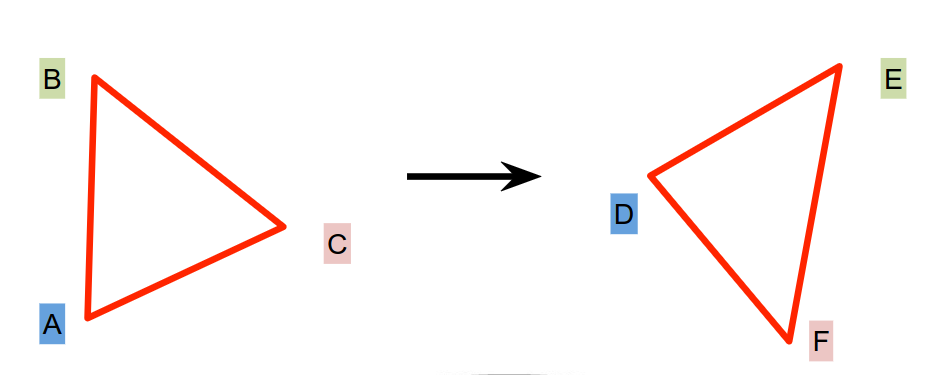
\includegraphics[width=0.5\linewidth]{images/part4/two-triangles.png}
\end{figure}

How do we determine which transformations were applied to $\Delta ABC$ to form $\Delta DEF$? That is, suppose all the points in ABC is $\mathrm{x}$, how do we determine the transformation $M$ such that
$$\mathrm{x}' = M\mathrm{x}$$

\textbf{Setup.} A 2D affine transform in homogeneous coordinates is
$$\begin{bmatrix}x'\\y'\\1\end{bmatrix} = \underbrace{\begin{bmatrix}a & b & t_x \\ c & d & t_y \\ 0 & 0 & 1\end{bmatrix}}_{M}\begin{bmatrix}x\\y\\1\end{bmatrix},$$
giving two scalar equations per correspondence:
$$x' = ax + by + t_x, \qquad y' = cx + dy + t_y.$$
There are 6 unknowns $(a,b,c,d,t_x,t_y)$, so \textbf{3 point correspondences} (6 equations) are necessary and sufficient --- exactly what a triangle provides.\\

\textbf{Linear system.} Stack the correspondences $A\!\to\!D$, $B\!\to\!E$, $C\!\to\!F$ into the system $P\,\mathbf{m} = \mathbf{q}$:
$$
\underbrace{
\begin{bmatrix}
x_A & y_A & 1 & 0   & 0   & 0 \\
0   & 0   & 0 & x_A & y_A & 1 \\
x_B & y_B & 1 & 0   & 0   & 0 \\
0   & 0   & 0 & x_B & y_B & 1 \\
x_C & y_C & 1 & 0   & 0   & 0 \\
0   & 0   & 0 & x_C & y_C & 1
\end{bmatrix}
}_{\mathbf{m}}
\begin{bmatrix}a\\b\\t_x\\c\\d\\t_y\end{bmatrix}
=
\begin{bmatrix}x_A'\\y_A'\\x_B'\\y_B\\x_D'\\y_D'\end{bmatrix}.$$

\textbf{Solution.} Since $P$ is $6\times6$ and non-singular (invertible) (provided the three source points are not collinear), the unique solution is $\mathbf{m} = P^{-1}\mathbf{q}$. Reconstruct $M$ from $\mathbf{m}$ and the fixed last row.

\emph{Note:} if the source points are collinear, $P$ is singular and the affine transform is underdetermined --- the triangle degenerates and no unique map exists.\\

\textbf{More than 3 points: exact vs.\ noisy.} With $n > 3$ correspondences, the system $P\mathbf{m} = \mathbf{q}$ is overdetermined ($P \in \mathbb{R}^{2n\times6}$). Two cases arise:

\begin{itemize}
  \item \emph{Noise-free data.} If all $n$ correspondences are exactly consistent with a single affine map (e.g.\ the corners of a square mapped to a parallelogram), then any 3 non-collinear points already determine $M$ uniquely, and every additional point is automatically satisfied --- the extra rows of $P$ are redundant. You can simply pick 3 points and solve the $6\times6$ system.
  \item \emph{Noisy data.} Real measurements have noise, so no single $M$ satisfies all equations simultaneously. The system is inconsistent and the best we can do is minimize the sum of squared residuals:
  $$\min_{\mathbf{m}}\;\|P\mathbf{m} - \mathbf{q}\|^2.$$
  The solution is given by the \textbf{normal equations}:
  $$P^T P\,\mathbf{m} = P^T\mathbf{q} \;\implies\; \mathbf{m} = (P^TP)^{-1}P^T\mathbf{q} = P^+\mathbf{q},$$
  where $P^+ = (P^TP)^{-1}P^T$ is the Moore--Penrose pseudoinverse. In practice, solve via QR decomposition or Singular Value Decomposition (SVD) rather than forming $P^TP$ explicitly.
\end{itemize}

The residual $\|P\mathbf{m}^* - \mathbf{q}\|$ measures how well an affine model fits the data; a large residual suggests the true transform is not affine (e.g.\ perspective distortion is present).



\NoteSection{3D Rotations}

\textbf{Rotation group $SO(3)$.} A 3D rotation is a $3\times3$ matrix $R$ satisfying $R^TR=I$ and $\det R=+1$. It has 3 DOF. Key representations:

\textbf{Rotation matrix.} Most natural for composing rotations ($R_3 = R_2 R_1$) and rotating vectors ($\mathbf{x}' = R\mathbf{x}$), but 9 numbers for 3 DOF - must maintain orthogonality constraints.\\

\textbf{Axis-angle / Rodrigues.} Any rotation is a rotation by angle $\theta$ about unit axis $\hat{\mathbf{n}}$. Let $[\hat{\mathbf{n}}]_\times$ denote the skew-symmetric cross-product matrix. Then:
$$R = I + \sin\theta\,[\hat{\mathbf{n}}]_\times + (1-\cos\theta)\,[\hat{\mathbf{n}}]_\times^2.$$
Compact (3 parameters: $\theta\hat{\mathbf{n}}$); numerically unstable near $\theta=0$ or $\theta=\pi$.\\

\textbf{Unit quaternion.} $q = (q_0, \mathbf{q}) = (\cos(\theta/2),\,\sin(\theta/2)\hat{\mathbf{n}}) \in \mathbb{R}^4$, $\|q\|=1$. Rotating a vector: $\mathbf{x}' = q\otimes(0,\mathbf{x})\otimes q^{-1}$. Composing two rotations: quaternion product $q_2\otimes q_1$. No gimbal lock; smooth interpolation via SLERP. $q$ and $-q$ represent the same rotation (double cover of $SO(3)$).\\

\textbf{3D Rigid Transform (6 DOF).} In homogeneous coordinates:
$$\begin{bmatrix}\mathbf{x}'\\1\end{bmatrix} = \begin{bmatrix}R & \mathbf{t}\\\mathbf{0}^T & 1\end{bmatrix}\begin{bmatrix}\mathbf{x}\\1\end{bmatrix}, \quad R\in SO(3),\;\mathbf{t}\in\mathbb{R}^3.$$
This is an element of $SE(3)$, the special Euclidean group. Composition is again matrix multiplication; inversion is $[R^T\;|\;-R^T\mathbf{t}]$.

\columnbreaknofill

\NoteChapter{Image Warping and Stitching}

\NoteSection{Image Warping}

Applying a geometric transformation to an image requires deciding how to compute pixel values at non-integer locations.\\

\textbf{Forward warping.} For each input pixel $(x,y)$, compute the output location $\mathbf{x}' = T(\mathbf{x})$ and write the value there.
\begin{itemize}
    \item Problem: output pixels can be \emph{missed} (holes) or \emph{overwritten} (conflicts) because the map from input to output is not one-to-one on the integer grid.
    \item Rarely used in practice.
\end{itemize}

\textbf{Inverse warping (preferred).} For each output pixel $\mathbf{x}'$, compute the source location $\mathbf{x} = T^{-1}(\mathbf{x}')$ in the input and interpolate:
$$g(\mathbf{x}') = f\bigl(T^{-1}(\mathbf{x}')\bigr).$$
Every output pixel is filled; no holes. Requires $T^{-1}$ to be available (always the case for the five transforms above).\\

% \textbf{Interpolation methods.} The source location $\mathbf{x} = (x,y)$ is generally non-integer.
% \begin{enumerate}
%     \item \textit{Nearest-neighbor.} Use $f(\lfloor x\rceil, \lfloor y\rceil)$. Fast but produces blocky artifacts.
%     \item \textit{Bilinear.} Let $(x_0,y_0) = (\lfloor x\rfloor, \lfloor y\rfloor)$, $\alpha = x - x_0$, $\beta = y-y_0$. Then
%     $$f(x,y) \approx (1{-}\alpha)(1{-}\beta)\,f_{00} + \alpha(1{-}\beta)\,f_{10} + (1{-}\alpha)\beta\,f_{01} + \alpha\beta\,f_{11}.$$
%     Smooth but slightly blurs edges. $C^0$ continuous (derivative discontinuities at integer boundaries).
%     \item \textit{Bicubic.} Fits a cubic polynomial through a $4\times4$ neighborhood. Sharper than bilinear; $C^1$ continuous. Standard in high-quality image editing pipelines.
% \end{enumerate}


\NoteSection{Interpolation for Inverse Warping}

When the inverse map $T^{-1}(\mathbf{x}')$ returns a non-integer location $(x,y)$, we cannot directly look up a pixel value. Interpolation reconstructs a continuous signal from the discrete grid so that the value at any real-valued coordinate can be estimated.

\NoteSubsection{Nearest-Neighbor Interpolation}

The output is assigned the value of the closest grid sample:
$$f(x,y) \approx f\!\left(\lfloor x\rceil,\, \lfloor y\rceil\right),$$
where $\lfloor\cdot\rceil$ denotes rounding to the nearest integer.
\begin{itemize}
    \item \textbf{Cost:} $O(1)$ — one table lookup.
    \item \textbf{Continuity:} $C^{-1}$ (piecewise constant; discontinuities at half-integer boundaries).
    \item \textbf{Artifacts:} Blocky/pixelated appearance, visible staircase edges on diagonal or curved features.
    \item \textbf{Use case:} Label maps, segmentation masks, or any application where the discrete class label must not be blended.
\end{itemize}

\NoteSubsection{Bilinear Interpolation}

Let $(x_0, y_0) = (\lfloor x\rfloor, \lfloor y\rfloor)$ be the integer floor, and define fractional offsets $\alpha = x - x_0$, $\beta = y - y_0 \in [0,1)$. The four surrounding samples are
\begin{align*}
    f_{00}&=f(x_0,y_0),\quad f_{10}=f(x_0{+}1,y_0),\\
    f_{01}&=f(x_0,y_0{+}1),\quad f_{11}=f(x_0{+}1,y_0{+}1).
\end{align*}

The bilinear estimate is obtained by first interpolating along rows, then along the column:
\begin{align*}
    f(x,\,y_0)   &= (1-\alpha)\,f_{00} + \alpha\,f_{10}, \\
    f(x,\,y_0{+}1) &= (1-\alpha)\,f_{01} + \alpha\,f_{11}, \\
    f(x,\,y)      &= (1-\beta)\,f(x,y_0) + \beta\,f(x,y_0{+}1).
\end{align*}
Expanding, the compact form is
$$f(x,y) \approx (1{-}\alpha)(1{-}\beta)\,f_{00} + \alpha(1{-}\beta)\,f_{10} + (1{-}\alpha)\beta\,f_{01} + \alpha\beta\,f_{11}.$$


Equivalently, in matrix form:
$$f(x,y) \approx
\begin{bmatrix}1-\alpha & \alpha\end{bmatrix}
\begin{bmatrix}f_{00} & f_{01}\\ f_{10} & f_{11}\end{bmatrix}
\begin{bmatrix}1-\beta\\ \beta\end{bmatrix}.$$


\begin{itemize}
    \item \textbf{Cost:} 3 lerps (or 4 multiplications + 3 additions per channel).
    \item \textbf{Continuity:} $C^0$ — the surface is continuous but its partial derivatives are discontinuous at integer boundaries.
    \item \textbf{Artifacts:} Mild blurring; no blocky artifacts. High-frequency detail is attenuated because the interpolating kernel (tent function) has a non-ideal frequency response.
    \item \textbf{Use case:} Default choice for image warping, texture mapping, and image resizing in real-time pipelines.
\end{itemize}

\NoteSubsection{Bicubic Interpolation}

Bicubic interpolation fits a degree-3 polynomial surface through a $4\times4$ neighborhood of 16 samples. The standard Keys cubic kernel with parameter $a=-0.5$ is
$$w(t) = \begin{cases}
(a+2)|t|^3 - (a+3)|t|^2 + 1 & 0 \le |t| < 1, \\
a|t|^3 - 5a|t|^2 + 8a|t| - 4a & 1 \le |t| < 2, \\
0 & |t| \ge 2.
\end{cases}$$
The interpolated value is
$$f(x,y) \approx \sum_{m=-1}^{2}\sum_{n=-1}^{2} f(x_0{+}m,\, y_0{+}n)\; w(m-\alpha)\, w(n-\beta).$$
\begin{itemize}
    \item \textbf{Cost:} 16 samples; separable — compute four cubic 1-D interpolations along $x$, then one along $y$ (12 multiplications per pass).
    \item \textbf{Continuity:} $C^1$ — both the function and its first derivatives are continuous.
    \item \textbf{Artifacts:} Slight ringing near sharp edges (Gibbs-like overshoot) due to the negative lobes of the kernel.
    \item \textbf{Use case:} High-quality image scaling, photo editing software, and medical imaging.
\end{itemize}

\NoteSubsection{Sinc / Lanczos Interpolation}

The ideal reconstruction filter for a band-limited signal is the sinc:
$$f(x,y) = \sum_{m}\sum_{n} f(m,n)\,\operatorname{sinc}(x-m)\,\operatorname{sinc}(y-n), \quad \operatorname{sinc}(t) = \frac{\sin(\pi t)}{\pi t}.$$
Because the sinc has infinite support it is truncated and windowed. The Lanczos-$a$ kernel multiplies sinc by a sinc-shaped window of radius $a$ (typically $a=2$ or $3$):
$$L_a(t) = \begin{cases} \operatorname{sinc}(t)\,\operatorname{sinc}(t/a) & |t| < a, \\ 0 & |t| \ge a. \end{cases}$$
\begin{itemize}
    \item \textbf{Cost:} $(2a)^2$ samples; $a=3$ requires 36 samples per output pixel.
    \item \textbf{Continuity:} $C^0$ at window boundary; approximately $C^\infty$ elsewhere.
    \item \textbf{Artifacts:} Best preservation of fine detail and frequency content; some ringing possible for $a=2$.
    \item \textbf{Use case:} Offline high-quality downsampling and super-resolution preprocessing.
\end{itemize}

\NoteSubsection{Comparison and Practical Guidelines}

\begin{center}
\begin{tabular}{lcccc}
\hline
\textbf{Method} & \textbf{Support} & \textbf{Continuity} & \textbf{Sharpness} & \textbf{Speed} \\
\hline
Nearest-neighbor & $1\times1$ & $C^{-1}$ & Highest (aliased) & Fastest \\
Bilinear         & $2\times2$ & $C^0$    & Medium             & Fast \\
Bicubic          & $4\times4$ & $C^1$    & High               & Moderate \\
Lanczos-3        & $6\times6$ & $\approx C^\infty$ & Highest (clean) & Slow \\
\hline
\end{tabular}
\end{center}

Key design decisions:
\begin{itemize}
    \item \textbf{Upsampling} (output larger than input): bicubic or Lanczos avoids the blurring of bilinear.
    \item \textbf{Downsampling} (output smaller than input): always \emph{anti-alias first} by low-pass filtering before sampling; otherwise all methods alias.
    \item \textbf{Discrete labels} (segmentation, depth maps): nearest-neighbor is mandatory to prevent blending across class boundaries.
    \item \textbf{Real-time constraints}: bilinear is hardware-accelerated in every GPU texture unit and is the pragmatic default.
\end{itemize}


\NoteSection{Panoramas and Image Stitching}


\begin{figure}[H]
    \centering
    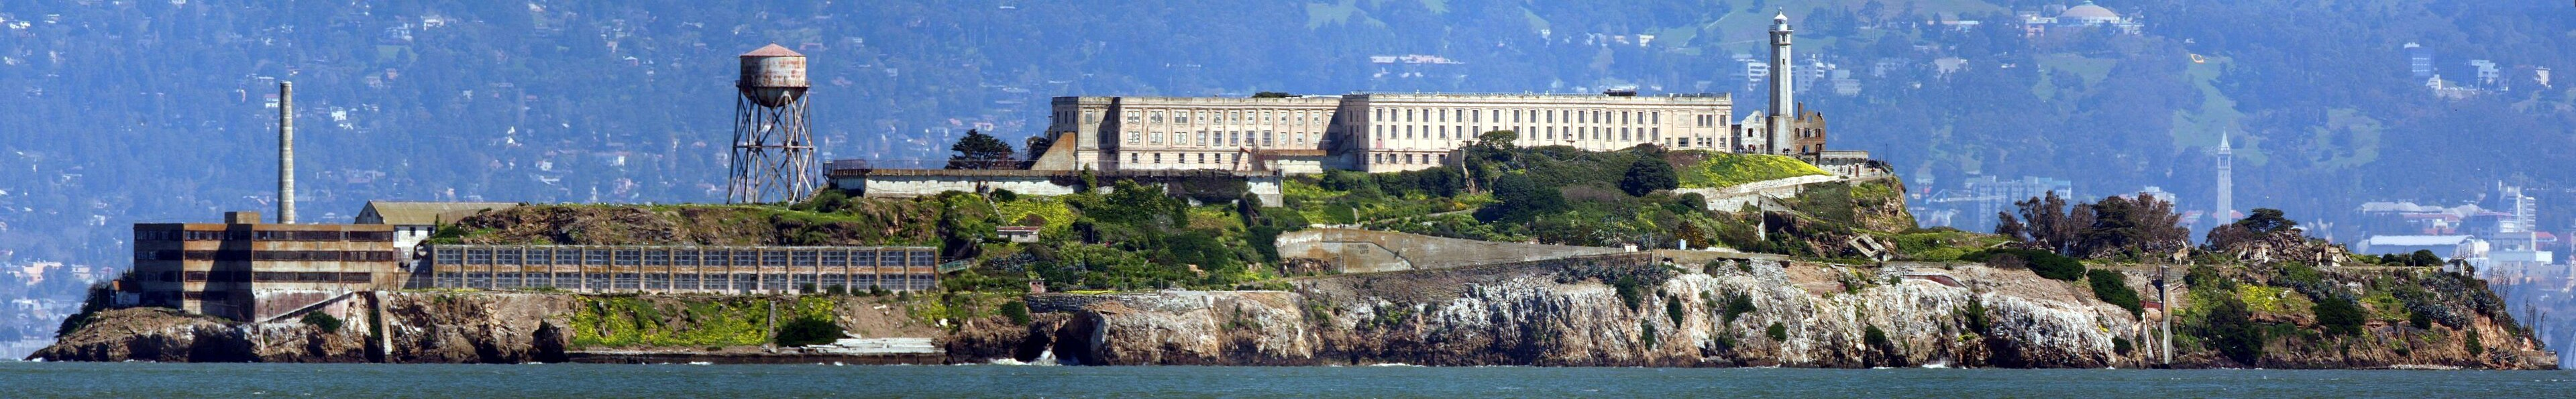
\includegraphics[width=1\linewidth]{images/part4/Alcatraz.png}
    \caption{Alcatraz Island, shown in a panorama created by image stitching}
\end{figure}

\textbf{Overview.} Panorama creation stitches overlapping photographs captured from (approximately) the same optical centre into a single wide-angle composite. Standard pipeline: \textbf{(1)} detect and match features across image pairs; \textbf{(2)} robustly estimate a homography per pair via RANSAC+DLT; \textbf{(3)} project all images onto a common surface (plane, cylinder, or sphere); \textbf{(4)} warp and composite; \textbf{(5)} blend seams. A homography relates two images whenever the camera undergoes a \emph{pure rotation} (fixed optical centre) or the scene is \emph{planar}.\\

\textbf{Homography Estimation - Direct Linear Transform (DLT).} Given $n \ge 4$ point correspondences $\{\mathbf{x}_i \leftrightarrow \mathbf{x}_i'\}$, DLT finds $H$ by forming a homogeneous linear system. Since $\tilde{\mathbf{x}}_i' \sim H\tilde{\mathbf{x}}_i$ (homogeneous equality), the cross-product condition
$$\tilde{\mathbf{x}}_i' \times H\tilde{\mathbf{x}}_i = \mathbf{0}$$
expands (for $\tilde{\mathbf{x}}_i=(x_i,y_i,1)^T$ and $\tilde{\mathbf{x}}_i'=(x_i',y_i',1)^T$) to two independent equations:
$$A_i\,\mathbf{h} = \mathbf{0}, \qquad A_i = \begin{bmatrix} \mathbf{0}^T & -\tilde{\mathbf{x}}_i^T & y_i'\,\tilde{\mathbf{x}}_i^T \\ \tilde{\mathbf{x}}_i^T & \mathbf{0}^T & -x_i'\,\tilde{\mathbf{x}}_i^T \end{bmatrix} \in \mathbb{R}^{2\times9},$$
where $\mathbf{h} = (h_{11},h_{12},\ldots,h_{33})^T \in \mathbb{R}^9$. Stacking all $n$ correspondences:
$$A\mathbf{h} = \mathbf{0}, \quad A\in\mathbb{R}^{2n\times9}.$$
The solution is the \emph{right singular vector} of $A$ for the \emph{smallest singular value} (via SVD), minimizing $\|A\mathbf{h}\|$ subject to $\|\mathbf{h}\|=1$. With $n=4$ correspondences $A$ is $8\times9$, the null space is one-dimensional, and $H$ is determined up to scale (8 DOF).

\begin{figure}[H]
    \centering
    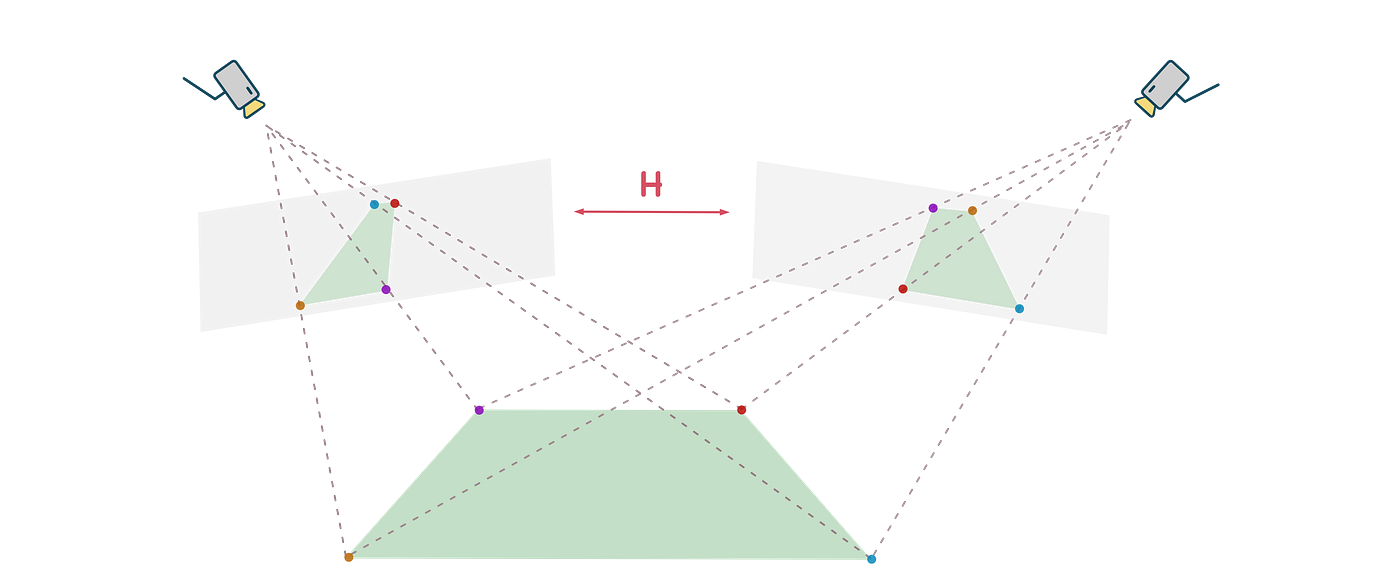
\includegraphics[width=0.75\linewidth]{images/part4/homography-estimation.png}
    \caption{Homography Estimation}
\end{figure}


\textbf{Normalization (essential).} Raw pixel coordinates (spanning hundreds to thousands of units) make $A$ severely ill-conditioned. Before forming $A$, independently normalize each point set:
\begin{enumerate}
    \item Translate so the centroid is at the origin: 
    $$\bar{\mathbf{x}}_i = \mathbf{x}_i - \boldsymbol{\mu}$$
    \item Scale uniformly so the mean distance from the origin is $\sqrt{2}$: 
    $$s = \sqrt{2}/\overline{\|\bar{\mathbf{x}}_i\|}$$
    \item The normalisation matrix is 
    $$T = \begin{bmatrix} s & 0 & -s\mu_x \\ 0 & s & -s\mu_y \\ 0 & 0 & 1 \end{bmatrix}$$
\end{enumerate}
Run DLT on $\hat{\mathbf{x}}_i = T\mathbf{x}_i$ and $\hat{\mathbf{x}}_i' = T'\mathbf{x}_i'$ to obtain $\hat{H}$; then denormalise: $H = T'^{-1}\hat{H}T$. Normalisation reduces condition numbers by orders of magnitude and is mandatory for numerical reliability (Hartley, 1997).\\

\textbf{RANSAC for robust estimation.} Descriptor matching yields many outliers. RANSAC applies with minimum sample $s=4$ (to fit $H$) and inlier threshold $\epsilon \approx 3$ pixels on reprojection error $\|\mathbf{x}_i' - H\mathbf{x}_i\|$. After RANSAC, refit $H$ on all inliers via DLT. Required iterations: $k = \log(1-p)/\log(1-(1-e)^4)$; for $e=0.5$, $p=0.99$: $k\approx72$.\\

\textbf{Non-linear refinement.} DLT minimises an \emph{algebraic} error with no geometric meaning. For higher accuracy, refine $H$ by minimising the \textbf{symmetric reprojection error}:
$$\min_H \sum_i \Bigl(d\!\left(\mathbf{x}_i',\,H\mathbf{x}_i\right)^2 + d\!\left(\mathbf{x}_i,\,H^{-1}\mathbf{x}_i'\right)^2\Bigr),$$
solved by Levenberg--Marquardt initialised from the DLT solution.\\

\textbf{Cylindrical projection.} For wide-angle panoramas ($>\!60°$ field of view), projective stitching produces severe distortion near the periphery. Instead, project each image onto a \emph{cylinder} of radius $f$ (focal length in pixels). For a point $(x,y)$ with origin at the image center:
$$\hat{x} = f\arctan\!\left(\tfrac{x}{f}\right), \qquad \hat{y} = \frac{fy}{\sqrt{x^2+f^2}}.$$
In cylindrical coordinates, a pure camera rotation about the vertical axis becomes a \emph{horizontal translation}, making alignment trivial for rotation-only sequences. The focal length $f$ must be known (from calibration or EXIF).\\

\textbf{Spherical projection.} For full $360°\times180°$ panoramas, project onto a sphere of radius $f$. Spherical angles of image point $(x,y)$:
$$\phi = \arctan\!\left(\tfrac{x}{f}\right), \qquad \lambda = \arctan\!\left(\tfrac{y}{\sqrt{x^2+f^2}}\right).$$
Re-project to \emph{equirectangular} (longitude--latitude) format: $(\phi,\lambda)\to(f\phi,\,f\lambda)$. Used in 360° video, VR headsets, and Google Street View.\\

\textbf{Image blending.} Warped images must be composited; seams appear due to exposure differences, vignetting, and sub-pixel misalignment.

\textit{Alpha feathering.} Assign each pixel a weight $w(\mathbf{x})$ proportional to its distance from the image boundary. In overlap regions blend linearly:
$$C(\mathbf{x}) = \frac{w_A(\mathbf{x})\,C_A(\mathbf{x}) + w_B(\mathbf{x})\,C_B(\mathbf{x})}{w_A(\mathbf{x}) + w_B(\mathbf{x})}.$$
Simple to implement; can produce ghosting under misalignment.

\textit{Multiband blending (Burt \& Adelson, 1983).} Low-frequency content should be blended with a wide transition (to hide color shifts); high-frequency content should be cut sharply (to preserve edge sharpness). Algorithm:
\begin{enumerate}
    \item Build Gaussian pyramids $G_A^{(\ell)}$, $G_B^{(\ell)}$ and mask pyramid $G_M^{(\ell)}$.
    \item Build Laplacian pyramids: $L_A^{(\ell)} = G_A^{(\ell)} - \mathrm{up}(G_A^{(\ell+1)})$, similarly $L_B^{(\ell)}$.
    \item Blend each level: $L_S^{(\ell)} = G_M^{(\ell)}\cdot L_A^{(\ell)} + (1-G_M^{(\ell)})\cdot L_B^{(\ell)}$.
    \item Collapse the blended Laplacian pyramid to reconstruct the composite.
\end{enumerate}

\textit{Seam finding (graph cut).} Rather than blending the entire overlap, find a \emph{minimum-cost cut} through the overlap where the two images agree most closely (minimum photometric difference). Kwatra et al.\ (2003) formulate this as a Markov Random Field and solve with graph cuts, eliminating ghosting entirely.\\

\textbf{Bundle adjustment for multi-image panoramas.} With $m>2$ images, composing pairwise homographies accumulates drift. Global alignment parameterises each camera by its rotation $R_i\in SO(3)$ and focal length $f_i$, then jointly minimises total reprojection error over all matched image pairs $(i,j)$ and inlier correspondences $k$:
$$\min_{\{R_i,\,f_i\}} \sum_{(i,j)\in\mathcal{E}}\;\sum_{k\in\mathcal{M}_{ij}} \left\|\mathbf{x}_k^{(j)} - \pi\!\left(R_j R_i^{-1}\,\pi^{-1}\!\left(\mathbf{x}_k^{(i)};\,f_i\right);\,f_j\right)\right\|^2,$$
where $\pi(\cdot;\,f)$ is projection with focal length $f$ and $\pi^{-1}$ back-projects to 3D. Solved by Levenberg--Marquardt (AutoStitch, Brown \& Lowe, 2007). \textbf{Gain compensation} (per-image exposure scale $g_i$) is typically added to the objective to handle photometric inconsistency between images.




\end{notes}
\end{document}
